\newpage
\section{動作実験}
%%%%%%%%%%%%%%%%%%%%%%%%%%%%%%%%%%%%%%%%%%%%%%%%%%%%%%%%%
\subsection{改良型細径羽状筋を備えたロボット}
3.2と4.1,4.2,4.3,4.4で述べた外骨格と羽状筋の設計方法と作製方法より開発した歩脚ロボットを図\ref{fig:kanirobot_new}に示す.
歩脚ロボットは長節,腕節,腕節,指節の4つの節で構成されている.
各節の内部には本研究で開発した改良型細径空圧羽状筋を備えている.
%%%%%%%%%%%%%%%%%%%%%%%%%%%%%%%%%%%%%%%%%%%%%%%%%%%%%%%%%
\subsection{動作実験}
本研究で開発した歩脚ロボットの改良型細径空圧羽状筋に圧縮空気を印加して,各関節の開閉動作および可動域を調べた.
関節の動きを確認しやすくするために長節-腕節間と前節-指節間は機体を寝かせた状態,腕節-前節間は機体を立てた状態で動作実験を行った.
また,初期位置は開筋か閉筋のどちらか一方が張った状態の位置にし,圧縮空気の印加は手動で行い印加圧力は 0.6MPa,開筋と閉筋の手動弁を交互に開閉することで動作させた.
ここで開筋は関節を開く方向に,閉筋は閉じる方向に作用する羽状筋を指す.

設計上の可動域と機体の可動域の比較を行うために,図\ref{fig:marker_jikki}のように各関節の軸となる部分にFDM方式の3Dプリンターで作製したマーカーを配置した.
マーカーをつけた状態で動作実験の様子を録画した.
その動画をトラッキングソフトの(kinovia)に読み込ませ,マーカーの1フレームごとの座標情報をxcelファイル形式で取得した.
そのxcelファイルの座標データをMATLABで読み込み,関節のマーカーから節端部のマーカーのベクトルと関節からもう一方の節端部のマーカーのベクトルを求めた.
その後,MATLABで先ほど求めたベクトルで内積を計算して脚の可動域を計算した.
%%%%%%%%%%%%%%%%%%%%%%%%%%%%%%%%%%%%%%%%%%%%%%%%%%%%%%%%%
\begin{figure}[ht]
    \begin{minipage}{0.49\hsize}
      \centering
      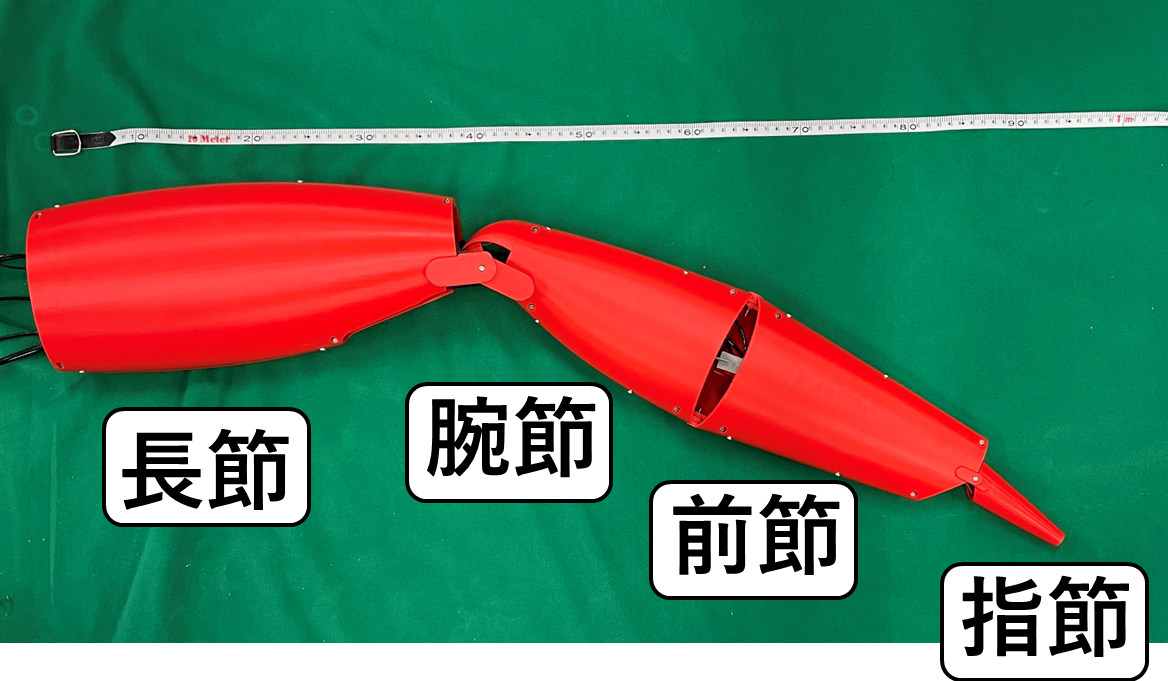
\includegraphics[scale=0.2]{image/jikki_2.png}
      \caption{本研究で作製した歩脚ロボット}
      \label{fig:kanirobot_new}
    \end{minipage}
    \begin{minipage}{0.49\hsize}
      \centering
      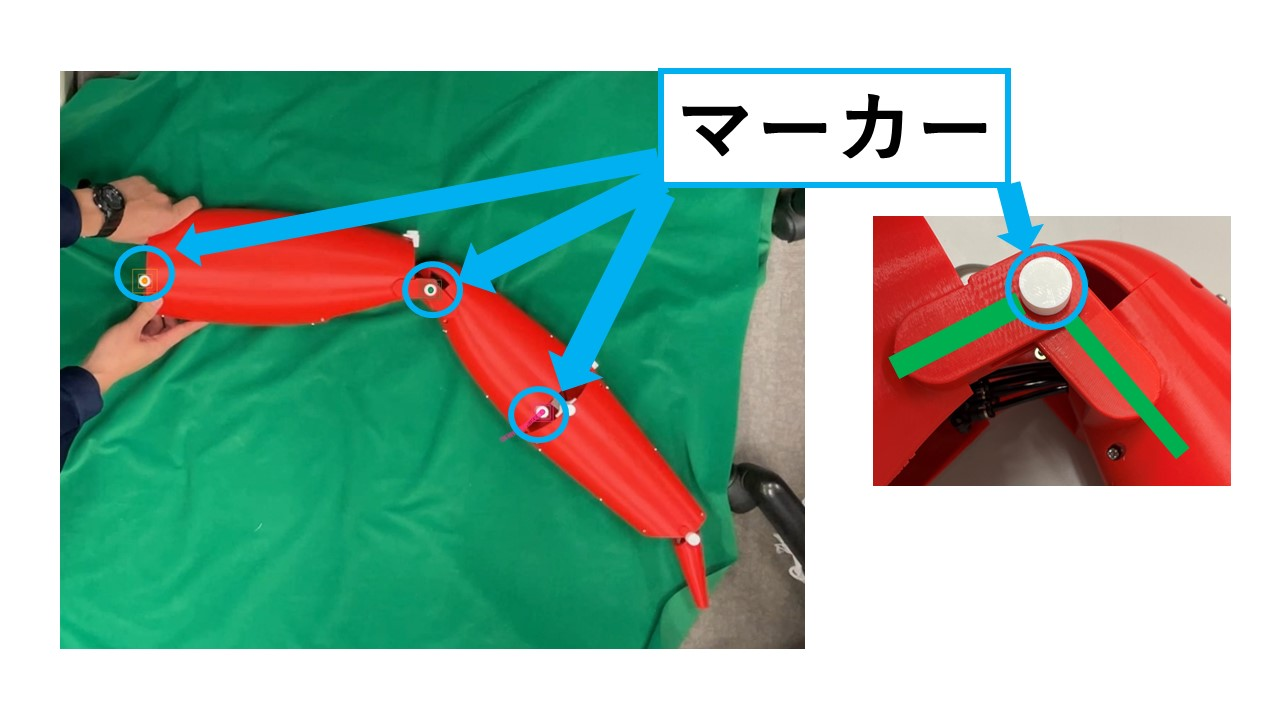
\includegraphics[scale=0.2]{image/marker.jpg}
      \caption{マーカーの配置の様子}
      \label{fig:marker_jikki}
    \end{minipage}
\end{figure}
%%%%%%%%%%%%%%%%%%%%%%%%%%%%%%%%%%%%%%%%%%%%%%%%%%%%%%%%%
\subsection{実験結果}
長節-腕節の動作実験を図\ref{fig:dousajikken}\subref{fig:move_1},腕節-前節の動作実験を図\ref{fig:dousajikken}\subref{fig:move_2},
前節-指節の動作実験を図\ref{fig:dousajikken}\subref{fig:move_3}に示す.
動作実験より,長節-腕節間では初期状態(図\ref{fig:dousajikken}\subref{fig:move_1}左)と最終状態(図\ref{fig:dousajikken}\subref{fig:move_1}右)では歩脚の角度が近い状態となった.
腕節-前節間,前節-指節間では長節-腕節間と同じような動作が見られたが,可動域が狭く感じられた.


実験の結果から可動域を算出したものを図\ref{fig:kadouiki_graph},表\ref{tab:kadouiki}に示す.
その結果,全ての関節において多少の誤差はあるものの,概ね設計通りの可動域が実現されていることが確認できた.
%%%%%%%%%%%%%%%%%%%%%%%%%%%%%%%%%%%%%%%%%%%%%%%%%%%%%%%%%
\begin{figure}[!ht]
    \begin{minipage}{1\hsize}
      \centering
      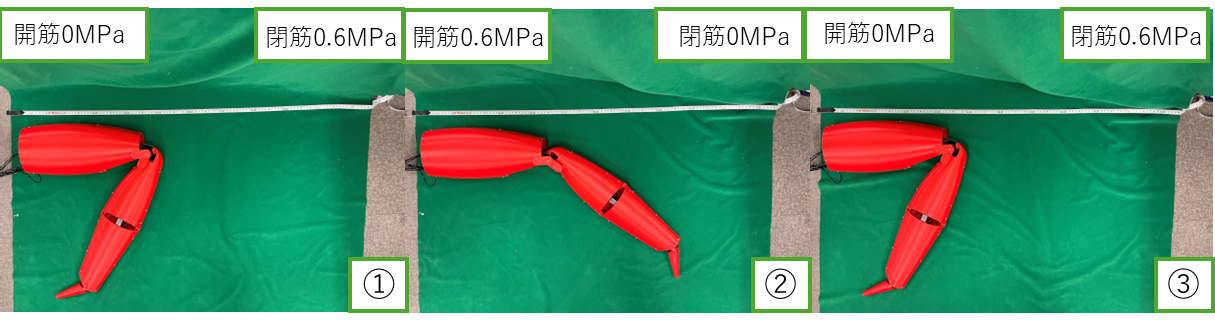
\includegraphics[scale=0.45]{image/chousetu-wansetu_edited.png}
      \vspace{-1mm}
      \subcaption{長節-腕節間の動作の様子}
      \label{fig:move_1}
    \end{minipage}
    %
    \begin{minipage}{1\hsize}
      \centering
      \vspace{3mm}
      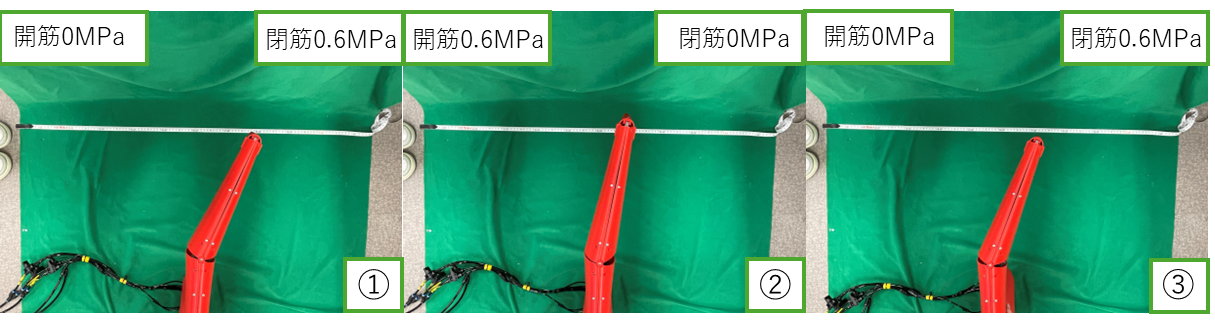
\includegraphics[scale=0.45]{image/wansetu-zensetu_edited.png}
      \subcaption{腕節-前節の動作の様子}
      \label{fig:move_2}
    \end{minipage}
    %
    \begin{minipage}{1\hsize}
      \centering
      \vspace{3mm}
      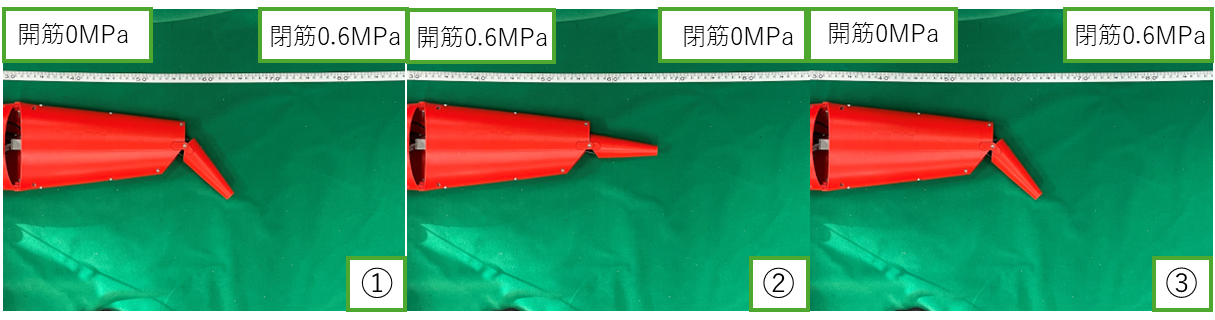
\includegraphics[scale=0.45]{image/zensetu-sisetu_edited.png}
      \subcaption{前節-指節の動作の様子}
      \label{fig:move_3}
    \end{minipage}
  \caption{動作実験の様子}
  \label{fig:dousajikken}
\end{figure}
%
\begin{table}[!ht]
    \centering
    \vspace{-2mm}
    \caption{実際の蟹と実機の可動域比較}
    \vspace{1mm}
    \scalebox{1.3}{ 
        \begin{tabular}{|c|c|c|c|}
            \hline
            項目/可動域[deg] & 長節-腕節間 & 腕節-前節間 & 前節-指節間 \\ \hline
            実際の蟹 & 52$\sim$130 & 0$\sim$45 & 0$\sim$89 \\ \hline
            計算上のロボット & 41.7$\sim$127.97 & 0$\sim$27 & 0$\sim$32.35 \\ \hline
            実際のロボット & 45.3$\sim$133.1 & 3.25$\sim$36.0 & 9.82$\sim$39.8 \\ \hline
        \end{tabular}
    }
    \label{tab:kadouiki}
\end{table}
%
\begin{figure}
    \centering
    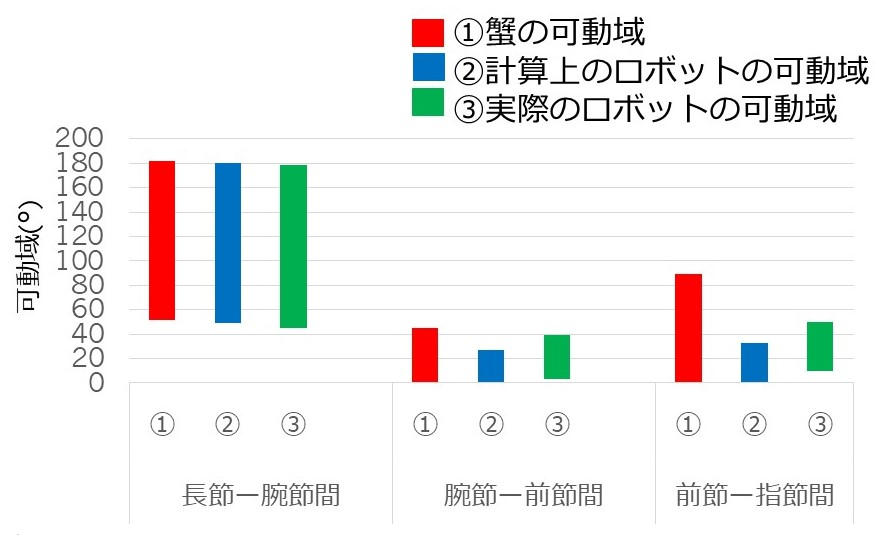
\includegraphics[scale=0.6]{image/kadouiki_graph.jpg}
    \caption{実際の蟹と実機の可動域比較}
    \label{fig:kadouiki_graph}
\end{figure}
%%%%%%%%%%%%%%%%%%%%%%%%%%%%%%%%%%%%%%%%%%%%%%%%%%%%%%%%%
\clearpage
\subsection{考察}
計算した可動域と実機の可動域で差が出た原因について考察する.
原因として,腱の固定方法が挙げられる.
図\ref{fig:ken_kotei},図\ref{fig:ken_kotei_moshiki}に本研究で作製した実機の腱の固定方法を示す.
本研究では腱をねじで押さえつけて固定する方法を採用した.
しかし,この固定方法では腱を設計通りの長さに固定することが難しく,計算上の腱の長さとの差が生じる可能性がある.
またTPU素材の腱は,柔軟であるが弾性を有するために曲げに対して復元力も生じる.
図\ref{fig:kadouiki_graph}を見てみると,実際のロボットの可動域が計算上のロボットの可動域と比べて閉じる方向にずれていることが確認できる.
これらの差により圧力を印加していない状態でも腱はわずかに引き込まれてしまい,計算上の可動域と実機の可動域の間に差が生じたと考えられる.

また本研究では,実機の可動域を計算するために数理モデルを用いたが,その数理モデルでは細径MPAを腱に固定する部品の高さを考慮していなかった.
実機と数理モデルの差を図\ref{fig:defference_model_jikki}に示す.
これにより計算上の細径MPAのストロークと差が出てしまったと考えられる.
この問題を解決するためには実機に近い構造を持つ数理モデルを構築し,それを用いてより正確な可動域を計算する必要があると考えられる.
%%%%%%%%%%%%%%%%%%%%%%%%%%%%%%%%%%%%%%%%%%%%%%%%%%%%%%%%%
\begin{figure}[ht]
    \begin{minipage}{0.49\hsize}
      \centering
      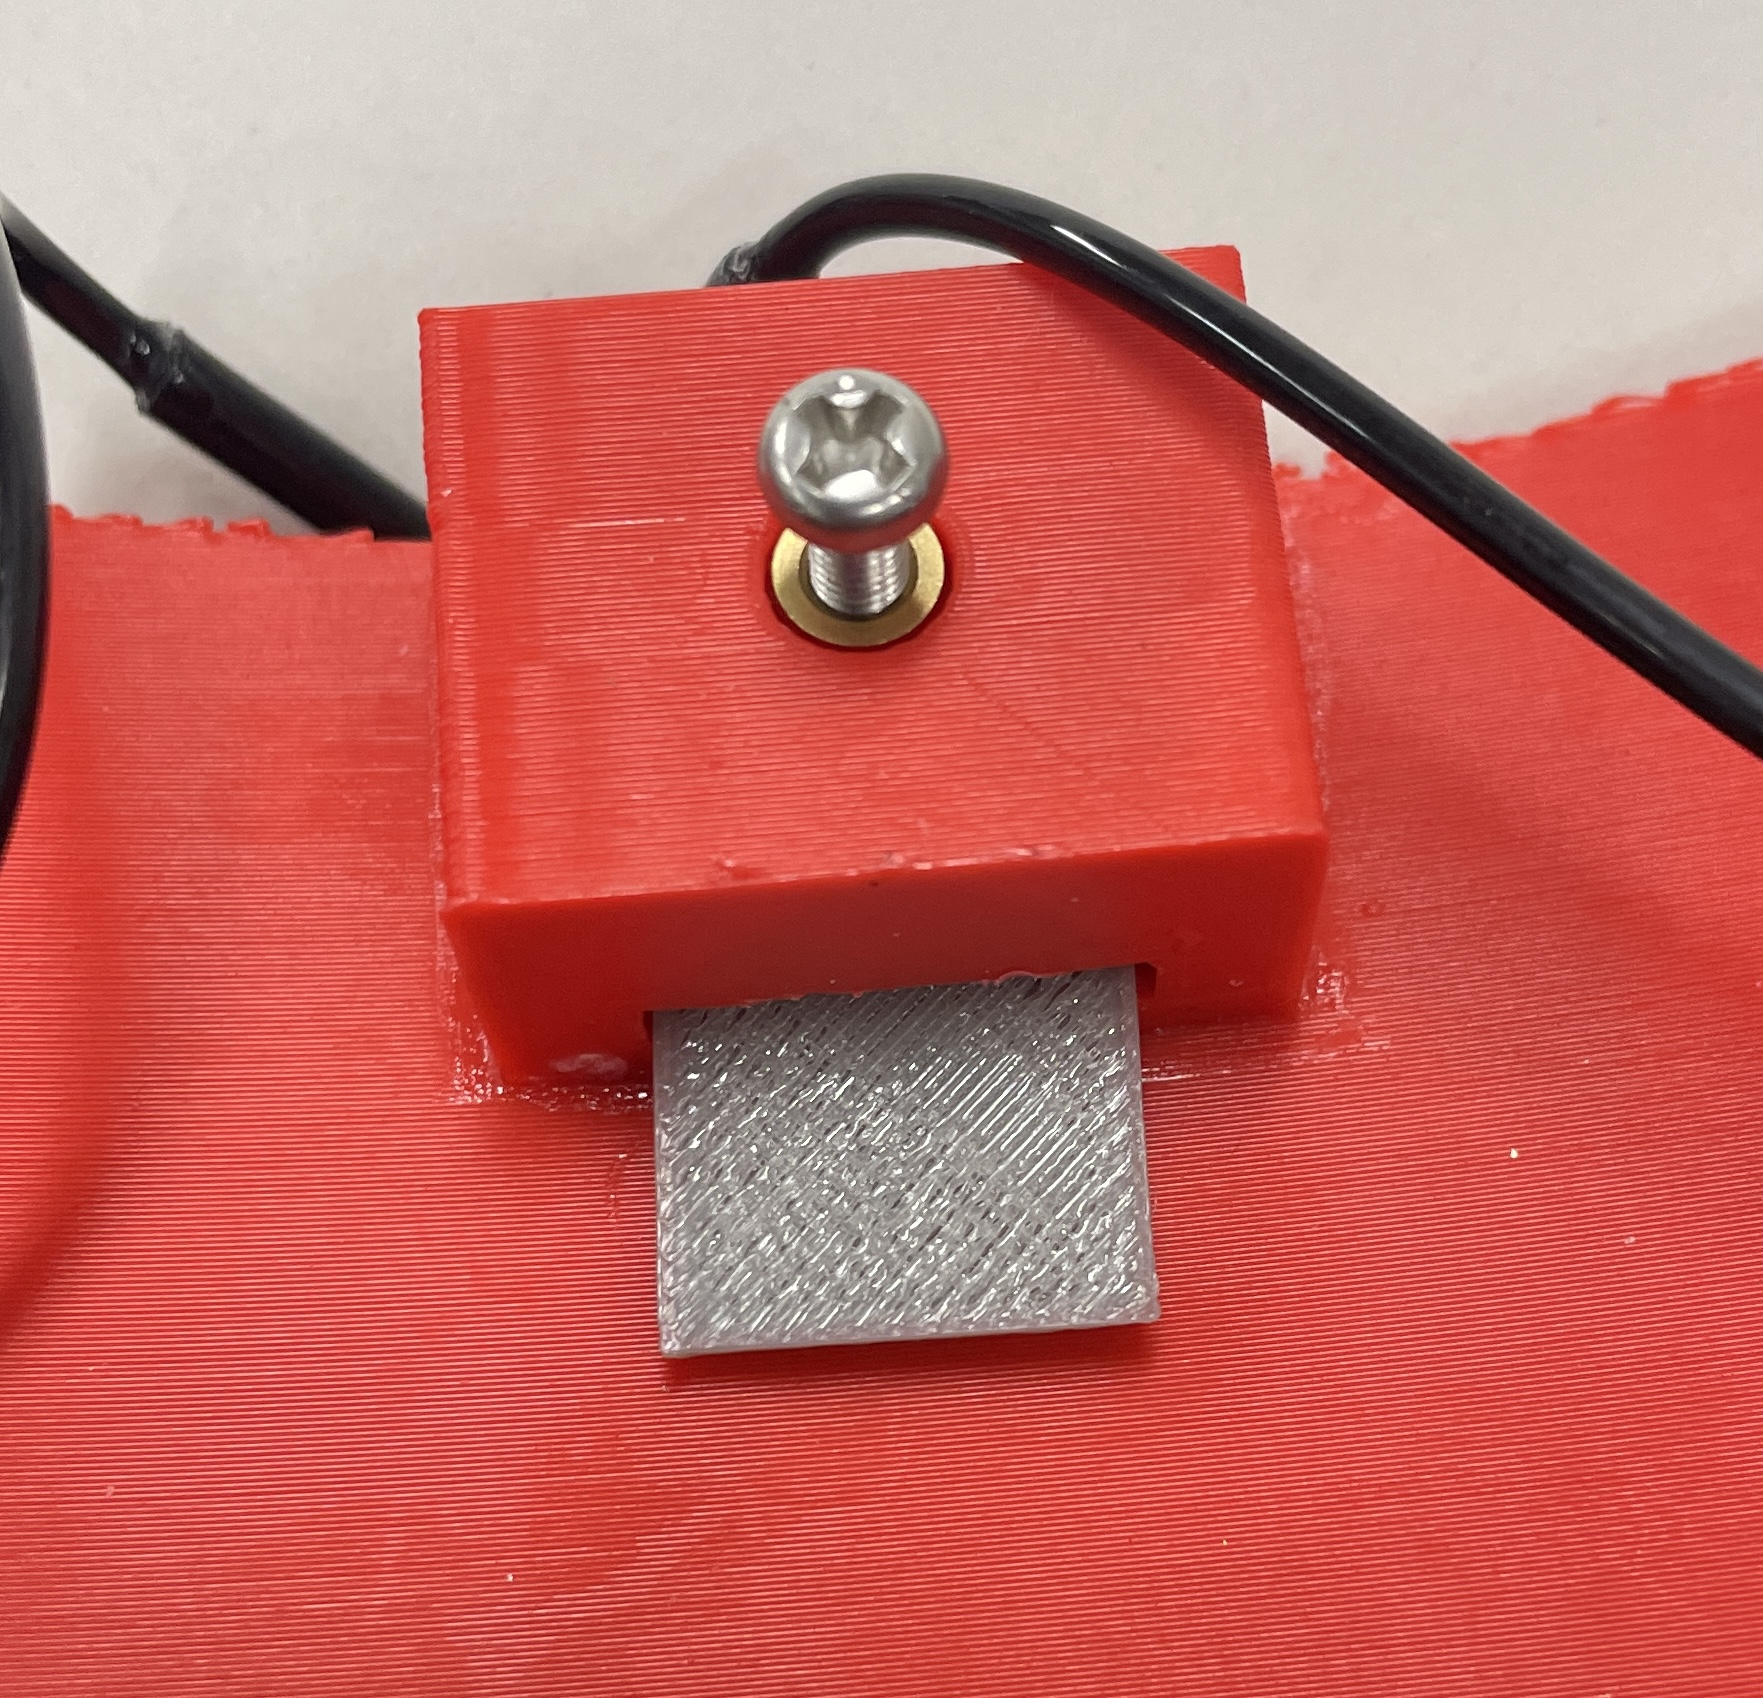
\includegraphics[scale=0.2]{image/kenkotei.jpg}
      \caption{腱の固定方法}
      \label{fig:ken_kotei}
    \end{minipage}
    \begin{minipage}{0.49\hsize}
      \centering
      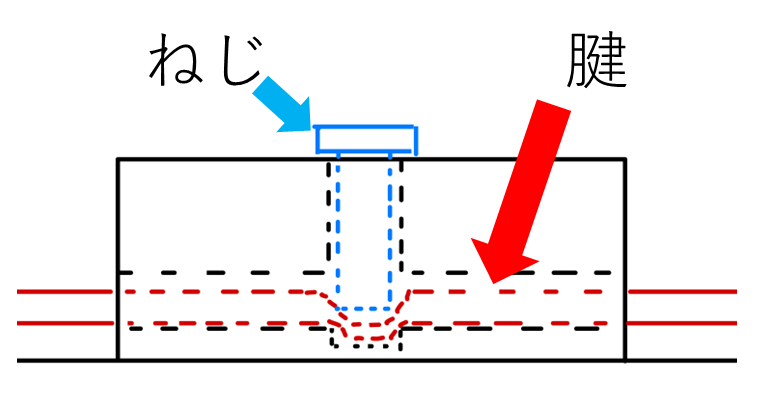
\includegraphics[scale=0.2]{image/moshiki_edited.png}
      \caption{腱の固定方法の模式図}
      \label{fig:ken_kotei_moshiki}
    \end{minipage}
\end{figure}
\begin{figure}[ht]
    \centering
    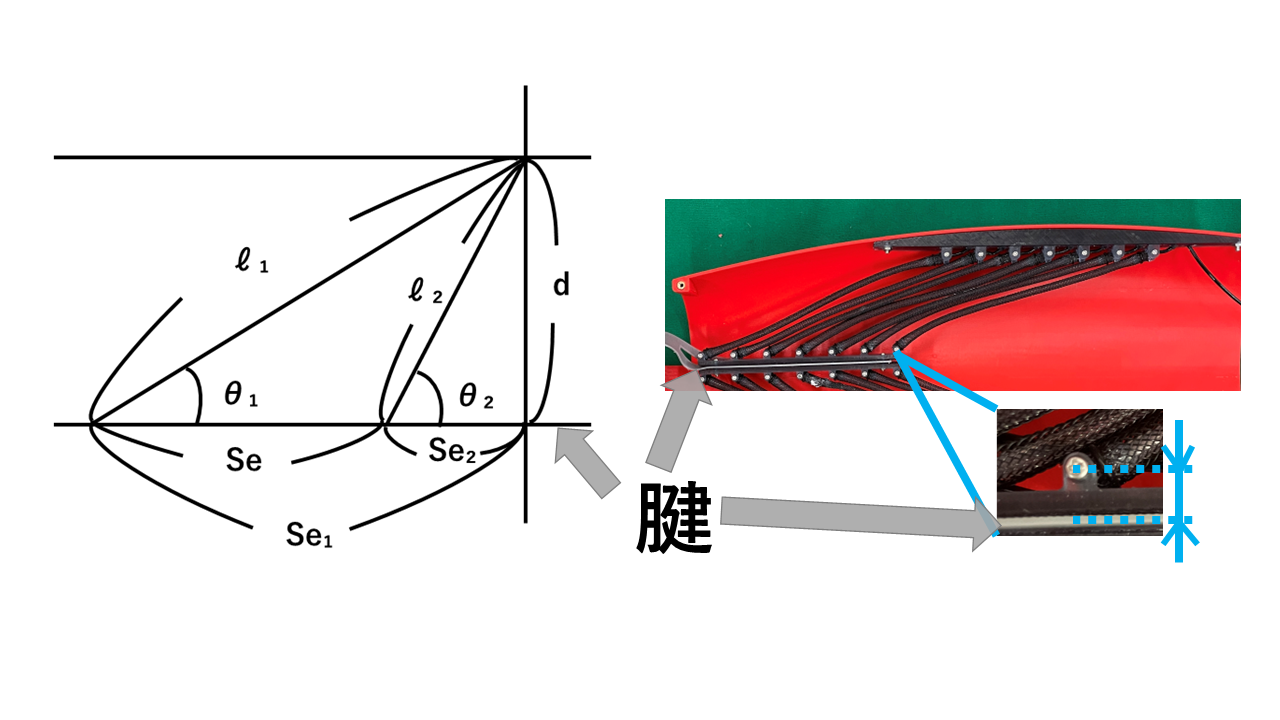
\includegraphics[scale=0.4]{image/model_jikki_defference.png}
    \caption{数理モデルと実機の差}
    \label{fig:defference_model_jikki}
\end{figure}